% -*- LaTeX -*-
% -*- coding: utf-8 -*-
%
% ~~~~~~~~~~~~~~~~~~~~~~~~~~~~~~~~~~~~~~~~~~~~~~~~~~~~~~~~~~~~~~~~~~~~~~~~~~~~~~
%
%                             michael a.g. aïvázis
%                      california institute of technology
%                      (c) 1998-2010  all rights reserved
%
% ~~~~~~~~~~~~~~~~~~~~~~~~~~~~~~~~~~~~~~~~~~~~~~~~~~~~~~~~~~~~~~~~~~~~~~~~~~~~~~
%

\lecture{Geometrical}{20100301}

% --------------------------------------
% contact detection
\begin{frame}[fragile]
%
  \frametitle{A more careful look at contact detection}
%
  \begin{itemize}
%
  \item consider a collection of tetrahedral meshes that model bodies in relative motion with
    triangular meshes as boundaries
%
  \item during the simulation, the bodies may come in contact
    \begin{itemize}
    \item with each other or themselves
    \item {\em contact events} consist of intersections among nodes, edges or faces
    \item unless the mechanics is informed of the contact events, the objects will
      inter-penetrate
    \item contact {\em detection} involves isolating the pairs of topological entities from
      each boundary that have intersected, whereas contact {\em resolution} refers to the
      calculation of appropriate restoring forces on the bodies
    \end{itemize}
%
  \item the typical simulation update step proceeds along the following lines
    \begin{enumerate}
    \item define the contact surfaces at time $t$
    \item predict the location of the nodes at a later time $t+\Delta t$ by integrating the
      equations of motion
    \item search for potential contact events among nodes, edges and faces to identify the
      entities that come in contact \label{item:contact-search}
    \item correct the future location of the nodes by applying forces that tend to remove the
      overlap
    \end{enumerate}
%
  \end{itemize}
%
\end{frame}

% --------------------------------------
% contact search
\begin{frame}[fragile]
%
  \frametitle{Contact search}
%
  \begin{itemize}
%
  \item the contact event identification in Step~\ref{item:contact-search} above has the
    potential to dominate the calculation
    \begin{itemize}
    \item given a candidate pair, the intersection logic involves very expensive geometrical
      calculations
    \item na\"ive algorithms are \order{n^{2}} in the number of topological entities on the
      boundary, prohibitively expensive even for moderate size calculations
    \end{itemize}
%
  \item hence, a more sensible strategy is to break up the contact search into two separate steps
    \begin{itemize}
    \item use a specialized data structure that encodes the location of mesh nodes and build a
      relatively fast algorithm to narrow down the candidates to a small number
    \item perform the detailed calculations on the reduced set
    \end{itemize}
%
  \item typically, the fast searches are implemented using {\em orthogonal range queries} that
    identify points whose co\"ordinates fall within a given box
    \begin{itemize}
    \item build a bounding box that contains the initial and final position of a given surface
      element, perhaps in some reduced form 
    \item form the {\em capture box} by enlarging the bounding box to account for the motion of
      the nodes
    \item query the data structure for nodes that fall within the capture box
    \end{itemize}
%
  \end{itemize}
%
\end{frame}

% --------------------------------------
% overview of contact
\begin{frame}[fragile]
%
  \frametitle{Orthogonal range queries}
%
  \begin{minipage}{.70\linewidth}
%
  \begin{itemize}
%
  \item an orthogonal range query is a generalization of the interval test to higher dimensions
    \begin{itemize}
    \item given a number $p$ and an interval $[a,b)$, return \keyword{true} if the number falls
    within the interval, otherwise return \keyword{false}
    \item extend by performing a test for each co\"ordinate: does the point $p$ fall within a
      given box?
    \end{itemize}
%
  \item there is a variety of data structures that are {\em a priori} well suited to this
    problem
    \begin{itemize}
    \item however, the problem context establishes some crucial constraints
    \end{itemize}
%
  \end{itemize}
%
  \end{minipage}
%
  \hfill
  \begin{minipage}{.27\linewidth}
    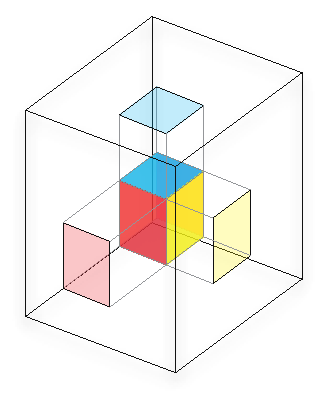
\includegraphics[scale=0.7]{figures/orq.pdf}
  \end{minipage} 
%
  \begin{itemize}
%
  \item we will classify algorithms according to the following metrics
    \begin{itemize}
    \item $b(N)$: the time it takes to initially populate the data structure with $N$ points
    \item $r(N)$: the complexity of rebuilding or update the data structure
    \item $s(N)$: the amount of storage required
    \item $q(N,n)$ and $\bar{q}(N,n)$: the (average) time required to perform a query if
      there are $n$ points in the given range
    \end{itemize}
%
  \item also, we'll start out in one dimension and generalize
%
  \end{itemize}
%
\end{frame}

% --------------------------------------
% simple algorithms
\begin{frame}[fragile]
%
  \frametitle{Sequential scan}
%
  \begin{itemize}
%
  \item the simplest approach is to look at each record and determine whether it falls in the
    range
    \begin{itemize}
    \item this algorithm is trivial to implement and requires no extra storage
    \item the performance is acceptable for sufficiently small $N$, or if most of the records
      fall in the query interval
      \begin{equation*}
        \begin{array}{rclcrcl}
          b_{{\tt SCAN}} & = & \order{N} &, &
          r_{{\tt SCAN}} & = & 0  \\
          s_{{\tt SCAN}} & = & \order{N} &, &
          q_{{\tt SCAN}} & = & \order{N}
        \end{array}
      \end{equation*}
    \end{itemize}
%
  \end{itemize}
%
  \begin{center}
    \begin{minipage}{.85\linewidth}
      \begin{algorithm}[H]
        \label{alg:rq-scan}
%
        \DontPrintSemicolon
        % \NoCaptionOfAlgo
        \SetAlCapHSkip{0ex}
%
        \caption{\rqscan(points, interval)}
%
        $candidates \leftarrow \emptyset$ \;
        \For{$point$ \In $points$}{
          \If {$point \in interval$} {
            $candidates.insert(point)$
          }
        }
        \Return{$candidates$}
%
      \end{algorithm}
    \end{minipage}
  \end{center}
%
\end{frame}

% --------------------------------------
% simple algorithms
\begin{frame}[fragile]
%
  \frametitle{Binary search}
%
  \begin{itemize}
%
  \item if the records are sorted, a binary search can locate any record with cost $\order{\log
      N}$, so in order to find all $p \in [a,b)$
    \begin{itemize}
    \item find the first point that satisfies $p >= a$
    \item and collect points in sequence while $p < b$
    \item simple analysis yields
      \begin{equation*}
        \begin{array}{rclcrcl}
          b_{{\tt BS}} & = & \order{N \log N} &, &
          r_{{\tt BS}} & = & \order{N} \\
          s_{{\tt BS}} & = & \order{N} &, &
          q_{{\tt BS}} & = & \order{\log N + n}
        \end{array}
      \end{equation*}
      since the records must be sorted initially, while rebuilding the data structure can be
      done in linear time since it is almost sorted
    \end{itemize}
% 
  \end{itemize}
%
  \begin{center}
    \begin{minipage}{.85\linewidth}
      \begin{algorithm}[H]
        \label{alg:rq-bs}
%
        \DontPrintSemicolon
        % \NoCaptionOfAlgo
        \SetAlCapHSkip{0ex}
%
        \caption{\rqbs(points, interval=(a,b))}
        \vspace{.5em}
%
        $candidates \leftarrow \emptyset$ \;
        $iterator \leftarrow \bslb(points, a)$ \;
        \While{$\star iterator \leq b$}{
          \If {$point \in interval$} {
            $candidates.insert(point)$
          }
        }
        \Return{$candidates$}
%
      \end{algorithm}
    \end{minipage}
  \end{center}
%
\end{frame}

% --------------------------------------
% using trees
\begin{frame}[fragile]
%
  \frametitle{Tricks with trees}
%
  \begin{itemize}
%
  \item alternatively, we can store the points at the leaves of a binary tree data structure
    \begin{itemize}
    \item each internal tree node acts has a {\em discriminator} that splits the data set into
      two subsets
    \item numbers less than the discriminator go to the left branch, the rest to the right
    \item once the population drops below some threshold, create a leaf node to hold the points
    \end{itemize}
%
%
  \item two sensible choices for the discriminator are
    \begin{itemize}
    \item the midpoint of the interval: yields a recursive subdivision of the interval
      \begin{itemize}
      \item also known as interval trees or {\em orthotrees}
      \item quadtrees in two dimensions, octrees in three
      \end{itemize}
    \item the median of the data set: partitions the data in subsets of equal size
      \begin{itemize}
      \item $kd$ trees
      \end{itemize}
    \end{itemize}
%
  \end{itemize}
%
\end{frame}

% --------------------------------------
% creating a binary tree
\begin{frame}[fragile]
%
  \frametitle{Creating a binary tree}
%
  \begin{center}
    \begin{minipage}{.85\linewidth}
      \begin{algorithm}[H]
        \label{alg:binary-tree}
%
        \DontPrintSemicolon
        % \NoCaptionOfAlgo
        \SetAlCapHSkip{0ex}
%
        \caption{\treemake(points)}
        \vspace{.5em}
%
        \If{$length[points] < tree.leafSize$}{
          $leaf \leftarrow tree.newLeaf()$ \;
          $leaf.insert(points)$ \;
          \Return{$leaf$}
        }\Else{
          $branch \leftarrow tree.newBranch()$ \;
          select branch $discriminator$ \;
          $left \leftarrow \left\{ x \in points : x < discriminator \right\}$ \;
          $branch.left \leftarrow tree.make(left)$ \;
          $right \leftarrow \left\{ x \in points : x >= discriminator \right\}$ \;
          $branch.right \leftarrow tree.make(right)$ \;
          \Return{branch}
        }
%
      \end{algorithm}
    \end{minipage}
  \end{center}
%
\end{frame}

% --------------------------------------
% range query in a binary tree
\begin{frame}[fragile]
%
  \frametitle{Querying a binary tree}
%
  \begin{center}
    \begin{minipage}{.85\linewidth}
      \begin{algorithm}[H]
        \label{alg:rq-tree}
%
        \DontPrintSemicolon
        % \NoCaptionOfAlgo
        \SetAlCapHSkip{0ex}
%
        \caption{\rqtree(tree, interval=(a,b))}
        \vspace{.5em}
%
        \If{$tree$ \Is $leaf$}{
          \Return{$\rqscan(tree.points, interval)$}
        }\Else{
          $candidates \leftarrow \emptyset$ \;
          \If {$tree.discriminator \geq a$} {
            $candidates \leftarrow candidates + \rqtree(tree.left, interval)$ \;
          }
          \If {$tree.discriminator < b$} {
            $candidates \leftarrow candidates + \rqtree(tree.right, interval)$ \;
          }
          \Return{$candidates$}
        }
%
      \end{algorithm}
    \end{minipage}
  \end{center}
%
\end{frame}

% --------------------------------------
% binary tree performance
\begin{frame}[fragile]
%
  \frametitle{Performance of binary trees}
%
  \begin{itemize}
%
  \item for midpoint splitting, the depth $D$ of the tree depends on the point distribution
    \begin{equation*}
      \begin{array}{lll}
        b_{{\tt ORTHO}} = \order{(D+1)N} &
        r_{{\tt ORTHO}} = \order{(D+1)N}  \\
        s_{{\tt ORTHO}} = \order{(D+1)N} &
        q_{{\tt ORTHO}} = \order{N} &
        \bar{q}_{{\tt ORTHO}} = \order{D+n}
      \end{array}
    \end{equation*}
%
  \item for median splitting the depth of the tree depends only on the number of records
    \begin{equation*}
      \begin{array}{ll}
        b_{{\tt KD}} = \order{N \log N} &
        r_{{\tt KD}} = \order{N}  \\
        s_{{\tt KD}} = \order{N} &
        q_{{\tt KD}} = \order{n + \log N}
      \end{array}
    \end{equation*}
%
  \end{itemize}
%
\end{frame}

% --------------------------------------
% binning in buckets
\begin{frame}[fragile]
%
  \frametitle{Binning}
%
  \begin{itemize}
%
  \item another strategy is to partition the interval $[a,b)$ into $M$ cells of width
    \[
    \delta \bydef x_{m+1} - x_{m} = \frac{b-a}{M}
    \]
    \begin{itemize}
    \item the \th{m} cell $C_{m}$ holds points in the interval $[x_{m}, x_{m+1})$
    \item the point container then becomes an array of $M$ point containers
    \item and the array index for a point $p$ is obtained through
      \[
      i = \lfloor \frac{p-a}{\delta} \rfloor
      \]
    \end{itemize}
%
  \item the process of putting the points in the container is known as a {\em cell sort}
%
  \item they are optimal when properly tuned
      \begin{equation*}
        \begin{array}{lll}
          b_{{\tt CELL}} = \order{N + M} &
          r_{{\tt CELL}} = \order{N + M} \\
          s_{{\tt CELL}} = \order{N + M} &
          q_{{\tt CELL}} = \order{J + n} &
          \bar{q}_{{\tt CELL}} = \order{n}
        \end{array}
      \end{equation*}
      where $J$ is the number of cells that overlap the query interval
%
  \end{itemize}
%
\end{frame}

% --------------------------------------
% range query in a cell array tree
\begin{frame}[fragile]
%
  \frametitle{Querying a cell array}
%
  \begin{center}
    \begin{minipage}{.85\linewidth}
      \begin{algorithm}[H]
        \label{alg:rq-cell}
%
        \DontPrintSemicolon
        % \NoCaptionOfAlgo
        \SetAlCapHSkip{0ex}
%
        \caption{\rqcell(cells, interval=(a,b))}
        \vspace{.5em}
%
        $candidates \leftarrow \emptyset$ \;
        $i \leftarrow index(cells, a)$ \;
        $j \leftarrow index(cells, b)$ \;
        \For{$point$ \In $cells[i]$}{
          \If{$point \geq a$}{
            $candidates.insert(point)$ \;
          }
        }
        \For{$k$ \In $[i+1 .. j-1]$}{
          \If{$point$ \In $cells[k]$}{
            $candidates.insert(point)$ \;
          }
        }
        \For{$point$ \In $cells[j]$}{
          \If{$point < b$}{
            $candidates.insert(point)$ \;
          }
        }
        \Return{$candidates$}
%
      \end{algorithm}
    \end{minipage}
  \end{center}
%
\end{frame}

% --------------------------------------
% higher dimensions
\begin{frame}[fragile]
%
  \frametitle{Generalizing to higher dimensions}
%
  \begin{itemize}
%
  \item the sequential scan algorithm has trivial generalizations
    \begin{itemize}
    \item its performance is only acceptable for very small numbers of points
    \item frequently used by the other algorithms to manage small size point sets
    \end{itemize}
%
  \item binary search generalizes to the {\em projection} method in $d$ dimensions
    \begin{itemize}
    \item sort the points according to their \th{k} co\"ordinate and build a reference set for
      this ordering
    \item for example, one can number the points, sort them according to each co\"ordinate, and
      build arrays of the point indices, or arrays of pointers to the actual data
    \item a range query along any dimension yields all the points that lie within a slice of
      the domain
    \item to perform an orthogonal range query
      \begin{itemize}
      \item perform a range query along each dimension using binary searches
      \item identify the co\"ordinate slice with the fewest records
      \item perform a sequential scan
      \end{itemize}
    \end{itemize}
%
  \end{itemize}
%
\end{frame}

% --------------------------------------
% kd tree
% s
\begin{frame}[fragile]
%
  \frametitle{$kd$ trees}
%
  \begin{itemize}
%
  \item in $d$ dimensions, there is a median point for each co\"ordinate
    \begin{itemize}
    \item split the tree using the co\"ordinate with the largest spread
    \item repeat this process at each level of the tree until the number of points to insert
      into the tree drops below some threshold
    \item every internal node of the tree has to record at least
      \begin{itemize}
      \item the direction that was chosen for the split
      \item the value of the discriminant
      \item references to the left and right branches of the node
      \end{itemize}
    \item leaf nodes are just point containers
    \end{itemize}
%
  \item the orthogonal range query is defined recursively
    \begin{itemize}
    \item at each internal node, check whether the left and right subdomains intersect the
      query interval by examining the discriminator
    \item recurse into the branches that intersect the range
    \item leaf nodes are examined using a sequential search
    \end{itemize}
%
  \end{itemize}
%
  \begin{figure}
    \begin{minipage}{0.75\linewidth}
    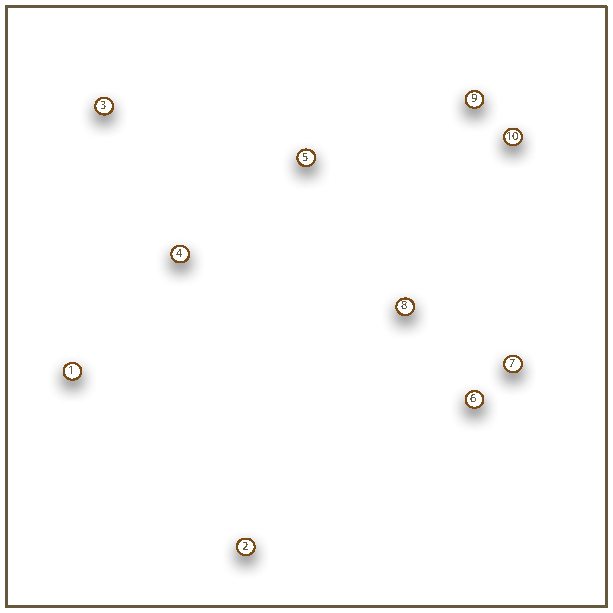
\includegraphics[scale=0.2]{figures/spatial-points.pdf}
    \hfill
    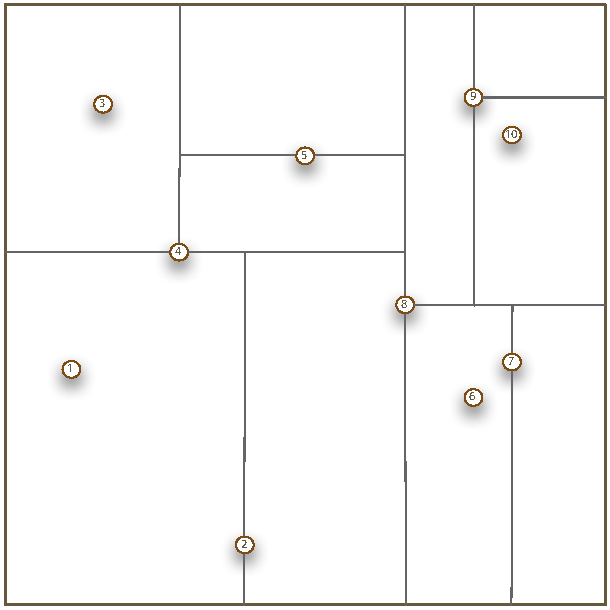
\includegraphics[scale=0.2]{figures/spatial-kd-split.pdf}
    \hfill
    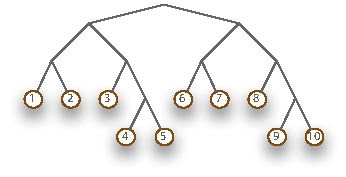
\includegraphics[scale=0.6]{figures/spatial-kd-tree.pdf}
  \end{minipage}
  \end{figure}
%
\end{frame}

% --------------------------------------
% orthotrees
\begin{frame}[fragile]
%
  \frametitle{Orthotrees}
%
  \begin{itemize}
%
  \item orthotrees are the generalization of interval trees in $d$ dimensions
    \begin{itemize}
    \item commonly known as {\em quadtrees} in two dimensions, and {\em octrees} in three
    \item recursively split the $d$-dimensional domain into $2^{d}$ equal size hyperboxes
    \item each internal node has $2^{d}$ branches
    \item some of the branches lead to leaf nodes that contain the actual data
    \end{itemize}
%
  \item the depth of the tree depends on the actual distribution of points in the input set
    \begin{itemize}
    \item points that are very close to each other could lead to some very deep trees
    \end{itemize}
%
  \item orthogonal range queries are implemented similarly to $kd$ trees
%
  \end{itemize}
%
  \begin{figure}
    \begin{minipage}{0.75\linewidth}
    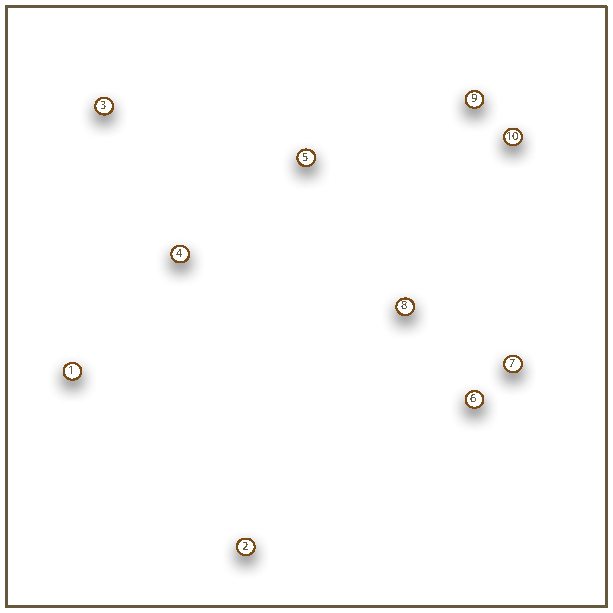
\includegraphics[scale=0.2]{figures/spatial-points.pdf}
    \hfill
    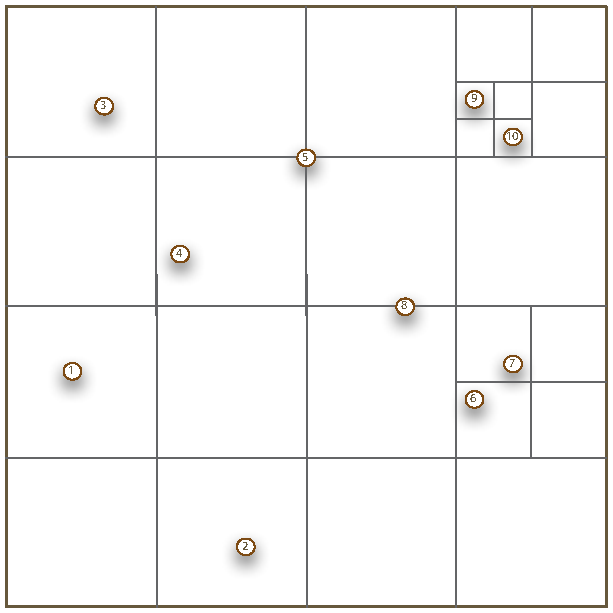
\includegraphics[scale=0.2]{figures/spatial-ortho-split.pdf}
    \hfill
    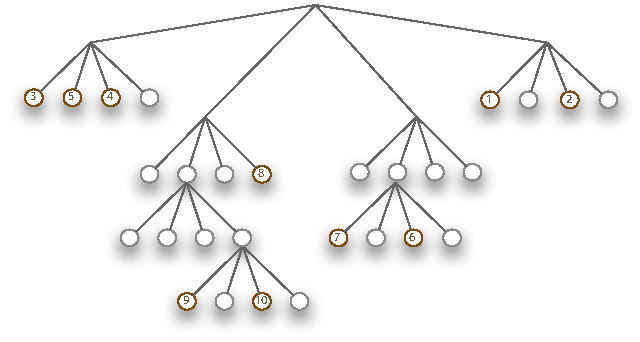
\includegraphics[scale=0.3]{figures/spatial-ortho-tree.pdf}
  \end{minipage}
  \end{figure}
%
\end{frame}

% --------------------------------------
% cells
\begin{frame}[fragile]
%
  \frametitle{Binning in higher dimensions}
%
  \begin{itemize}
%
  \item cell sort extends naturally to $d$ dimensions
    \begin{itemize}
    \item form a regular grid of spacing $\delta_{i}$ along the \th{i} dimension
    \item convert the point coordinates into cell indices along each dimension using the same
      formula as in one dimension
    \end{itemize}
%
    \item the orthogonal range query consists of accessing cells that
      \begin{itemize}
      \item entirely interior to the query box
      \item partially overlap the boundary of the query box
      \item the former are unconditionally included in the candidate list, while point in the
        latter must be checked individually
      \end{itemize}
%
    \item tuning is crucial to the performance of this method
      \begin{itemize}
      \item cells that are too large can lead to many false positives
      \item cells that are too small have higher access times
      \item it is best to know the size of the query boxes so that the cell spacing can be
        optimized
      \end{itemize}
%
    \item can be easily combined with any of the other methods to speed up access to the points
      in each cell
      \begin{itemize}
      \item most combinations do not offer significant advantages
      \item but using binary searches is an exception
      \end{itemize}
%
  \end{itemize}
%
\end{frame}

% --------------------------------------
% parallelization
\begin{frame}[fragile]
%
  \frametitle{Parallelization}
%
  \begin{itemize}
%
  \item minimization of the communication cost
    \begin{itemize}
    \item best to avoid communication altogether if possible
    \item any type of globally distributed data structure would eventually dominate the
      calculation
    \item so would global data exchanges to maintain locally consistent information
    \end{itemize}
  \item load balancing
    \begin{itemize}
    \item the parallel characteristics of contact are different from the solver update
    \item it is probably unavoidable that a few processors will be responsible for detecting and
      resolving the bulk of contact
    \end{itemize}
%
  \item utilize point-to-point communications as much as possible
    \begin{itemize}
    \item build/exchange bounding boxes for the geometry kept by each processor
    \item use it to build point-to-point communication maps
    \item exchange boundary elements so contact resolution can happen locally
    \item exchange the resulting forces
    \end{itemize}
%
  \item a research problem
    \begin{itemize}
    \item we know that processing multiple queries has better parallel characteristics than a
      single one
    \item we need a self-balancing, dynamically repartitioning data structure
    \end{itemize}
%
  \end{itemize}
%
\end{frame}


% end of file 
